%% Background Theory
%%=========================================

\chapter{Background Theory}
\label{ch:background}
While many problems may seem similar in nature, small factors can influence how a problem has to be solved. Some factors even influence the problem so much that it becomes a completely different one. This chapter investigates what type of problem we are trying to solve. In this chapter we will look at theory relevant to the the underlying structure of our problem. We will evaluate what we want out system to read, and what we want our system to output. In section \ref{sec:natural_language_processing}, we will look at Natural Language Processing and how our problem can be considered as the task of machine translation.

%%=========================================

\section{Evaluating Problem Input and Output}
In our particular problem we have a input that is a matrix or a vector of binary data. The binary input denotes the color of a particular pixel at the given location in our ``signature". We want the output to be what character(s) the matrix or vector is made out of. For example, if our characters are the upper cased letters in the English language, we could want our output to be in the range 1 to 26, denoting A to Z. 

\begin{figure}[h]
    \begin{equation}
        \label{eq:input_output_example}
        \begin{aligned}
           \vec{\text{rawInput}}        &= \lbrack 4W, 3B, 7W, 3B, 8W, 3B, 18W, 3B, 23W, 3B, 13W, 14B, 6W, 3B, 10W, 3B \rbrack \\
           \vec{\text{encodedInput}}    &= \lbrack 4, -3, 7, -3, 8, -3, 18, -3, 23, -3, 13, -14, 6, -3, 10, -3 \rbrack \\
           \vec{\text{output}}          &= \lbrack 1, 12, 12, 9, 5, 4 \rbrack \\
           \text{word}                  &= \text{ALLIED}
        \end{aligned}
    \end{equation}
    \captionsetup{labelformat=empty}
    \caption{Input and output example}
\end{figure}

\ref{eq:input_output_example} contains an example with inputs and outputs for the word ``ALLIED". Note that in this example, we have also encoded the input to whole integers. We did this by negating the lengths of sequences of black pixels. This means that four black pixels are encoded as $-4$. Similarity, sequences of white pixels were not altered, so 18 white pixels would be encoded as $18$. This encoding was done to have easier data to work with. 

\subsection{Input Format}
Our input has the feature that they form a sequence. Both the values in the sequence, and the ordering of the sequence is crucial for prediction. This is fundamentally different from other problems such as traditional image recognition, where the exact location of a pattern is not important \red{cite}.

Because the input forms a sequence, it is important that the entire sequence is read, and that we do not cut the sequence off at the end, removing important information that we need. Truncating or ignoring a values in the input sequence would result in mislearning. Instead of our model correctly identify subsequences that result i a single output value, the model attempts to find patters in the data that is not there. This would cripple the model and the overall accuracy may suffer due to contradicting sequences.

\begin{figure}[h]
    \begin{equation}
        \label{eq:input_stop_words}
        \begin{aligned}
           \vec{\text{encodedInput}}        &= \lbrack -3, 23, \pi, -3, 13, \pi, -14, \pi \rbrack \\
           \text{word}                      &= \text{LIE}
        \end{aligned}
    \end{equation}
    \captionsetup{labelformat=empty}
    \caption{Input with stop words}
\end{figure}

We do also lack the concept of ``stop words" in our problem. Example \ref{eq:input_stop_words} illustrates an input with stop words, denoted as $\pi$. Using stop words may make the problem easier to solve, as as we would know within which boundaries each character resides. In example \ref{eq:input_stop_words}, we have placed the stop word right before the beginning of a new character, instead of just the barriers of the character itself. This could potentially reduce ambiguity as we would now know for a fact that the letter I, if followed by an E, would always be the subsequence $[-3, 13]$. Instead of relying on stop words, we want our model to find a pattern in the sequence data that makes sense based on the corresponding output. This pattern, if correctly predicted, would not need explicit stop words, as the model should be able to find them implicitly.

\subsection{Output Format}
As with the input, our output also form a sequence. Both the values in the sequence, and the ordering of the sequence, is important. The words `HELLO` and `HLLOE` contains the same letters, but have a different meanings. Understanding that both the individual values in the output sequence, as well as the placement of each of them, is important for understanding how our problem is different from many others.

%%=========================================

\section{Translation}
We have now considered the input and output separately. Considering them ``together" we can see the relationship between the two. Sequences and subsequences in the output results in an output sequence or single output value. We can look at this process as a type of translation. We ``translate" the input sequences of language $\alpha$ into a output sequence of language $\beta$. It is irrelevant that the actual input and output are not defined language with linguistic properties. As long as there is a relationship between the two ``languages", the task may be considered as a type of translation between them. Figure \ref{fig:number_translation} illustrates the translation between our two languages, reusing the data from Example \ref{eq:input_stop_words}. 

\begin{figure}[h]
    \centering
    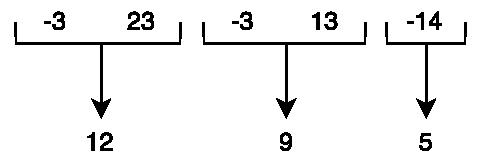
\includegraphics[width=0.7\textwidth]{fig/background_theory/number_translation.pdf}
    \caption{Illustrative translation between our two languages}
    \label{fig:number_translation}
\end{figure}